The simulation framework aims to simulate different simulation scenarios based on supplied configuration files.
To be able to trust in the results of  such a simulation, the outcome needs to be similar to each repeating execution of particular ticks.
During a simulation run, the different nodes are not synchronised in any manner, and the orchestrated containers run entirely independently from each other.
For example, the order of low-level operations executed by the different nodes on the host machine depends on many various parameters and circumstances, like for example random behaviour in the reference client, and is likely to change in every simulation run.
This indeterminism introduced by how the simulation framework works is unchangeable without breaking the whole architecture of the simulation framework.
Hence, the results of multiple executions of a particular tick sequence are only  evaluated against a specific similarity and not if the outcome is exactly the same.

\section{Near-Deterministic behaviour} \label{chap:deterministic_behaviour}
\aju{I would suggest to introduce a new term e.g., \emph{near-deterministic} to highlight that it is something different. 
Must not be that term but I did not came up with a better one. Would suggest a search/replace for that term}

The simulation framework is assessed against a defined \emph{near-deterministic} behaviour to have confidence in single executions of particular simulation scenario.
The software is considered to behave deterministically if:

%The standard deviation of the stale block rate is lower than 0.2\% after sufficient executions of the reference scenario.
The standard deviation of the stale block rate is lower than 0.2\% after 100 executions of the reference scenario.
\aju{What is \emph{sufficient}, I would write a specific value - also a small if not tested for larger ones but better be precise here.}

In this definition solely the stale block rate is used to define a deterministic behaviour because it reflects the outcome of a simulation comprehensively.
All configuration parameters of a simulation run influence the stale block rate directly or indirectly\cite{gervais2016security}:

\begin{itemize}
	\item The tick sequence reflects the computational share of the nodes and the block interval time of the overall network. Changes to the tick sequence yield in less or more block races in the peer-to-peer network.
	The stale block rate condenses the outcome of these block races.
	\item The latency in the peer-to-peer network directly influences the propagation time of blocks.
	With lower latency nodes can faster adopt the currently highest available block, where on the other hand with higher latency nodes more likely create competing blocks and cause block races.
	The block races are causing then stale blocks reflected by the stale block rate.
	\item The network topology defines how the peer-to-peer network is connected.
	Hence, the topology impacts how fast or slow blocks are propagating in the network which impacts the stale block rate.
\end{itemize}

%The definition of the deterministic behaviour is subjective and needs to be considered when trying to conclude something from the results of a simulation framework with such a deterministic behaviour.
%\aju{Would drop that sentence - confuses more than it helps I guess and it is clear now anyway that it is not 100% deterministic}

\section{Reference scenario}
\label{chap:reference_scenario}

The reference scenario used to evaluate the simulation framework for its deterministic behaviour, tries to abstract the real Bitcoin network.
The mining process in the real system is known to be dominated by a few mining pools \cite{gervais2014bitcoin, beikverdi2015trend, tschorsch2016bitcoin, clarkresearch, gencer2018decentralization}.
Current statistics show that about twenty miners create almost all blocks \cite{gencer2018decentralization, blockchaininfopools, coindanceblocks, bitcointickerpools}.
Hence, in the reference scenario, a total of twenty nodes are used.
These nodes are all directly connected to each other with a latency of 25 milliseconds.
The configuration of network topology with direct, fast connections is based on the assumption that every miner wants to hear about new blocks as fast as possible.
The rapid propagation time of the blocks reduces the number of stale blocks for each participating peer and thus, increases the revenue gained from the block rewards.
For the latency of the connections additionally an upper bound from previous research was taken into account \cite{decker2013information}.

For the sake of simplicity all nodes part of the network run the same version 0.15.0.1 \cite{bitcoin15} of the Bitcoin reference implementation.
This adjustment is in contrast to the real network where different implementation and version are used \cite{coindancenodes}.
Another simplification is taken for the virtual distribution of the computational power in the system.
In the reference scenario, all participating nodes  receive the same amount of computational power.
Consequently, the probability that a node finds the next block is the same for every particular node at every point in time.
In the real network, the distribution of the computational power is unevenly, and about five mining pools mine over fifty percent of all blocks \cite{gervais2014bitcoin, blockchaininfopools, coindanceblocks, bitcointickerpools}. 

The duration of the simulation itself is set to contain about 2016 blocks which correspond to two weeks in the real Bitcoin network.
This time span is also identical to the time used for the difficulty adjustment of the proof-of-work in Bitcoin which is relevant for the simulation of selfish mining. 
The needed tick sequence is generated by using the \textit{ticks} command described in section \ref{chap:ticks_command}.
The command uses an exponential distribution to determine when a specific node should find a block. 
The exponential distribution realistically mimics the block intervals caused by the cryptographic proof-of-work puzzle normally executed by every node to search a new block \cite{nakamoto2008bitcoin, decker2013information, eyal2014majority}.
In the reference scenario, the simulation is divided into 0.1 second long ticks.
Hence, by setting the blocks per tick to $0.0\dot{3}$, the simulated network finds every three seconds a block.
Compared to Bitcoin, wherein average every ten minutes a block is created, this results in a 200 times shorter block interval, and instead of two weeks, it takes 100.8 minutes to simulate about 2016 blocks.

\section{Evaluation}
\label{chap:evaluation}

For the evaluation of the deterministic behaviour the reference scenario was executed 100 times to obtain sufficient figures of the stale block rate.
The individual simulations were conducted on an \textit{x86 Linux} host machine with \textit{Ubuntu 4.4.0-97-generic} installed.
The CPU of the host machine was virtualised with \textit{QEMO 2.5+} and provided 16 cores.
Furthermore, the machine provided 57.718 GB of memory.
During a particular simulation run, about 4\% of CPU and 6\% of the storage were utilised as shown in the corresponding figures \ref{fig:cpu_usage} and \ref{fig:storage_usage}.
The metrics about the usage of the CPU and storage were continuously collected by the simulation framework as described in chapter \ref{chap:commands}.

The outcome of the evaluation is shown as box plot in figure \ref{fig:box_stale_rate} and as a density plot in \ref{fig:density_stale_rate}.
Despite one outlier at 4.521\% all data points are inside the whiskers area defined by $[Q1 - 1.5IQR, Q3 + 1.5IQR]$ with the median value equal 4.821\%.
Even though the stale block rate is a continuous variable, the calculated 100 values are accumulated at certain values because the fixed amount of blocks only allows certain combinations of accepted and stale blocks.

To evaluate if the simulation framework has a deterministic behaviour as defined in chapter \ref{chap:deterministic_behaviour} the standard deviation is calculated.
The calculation of the standard deviation results in 0.159\%.
Hence, the value satisfies the defined deterministic behaviour, and the simulation framework can be assumed to behave deterministically as defined.

\begin{figure}[t]
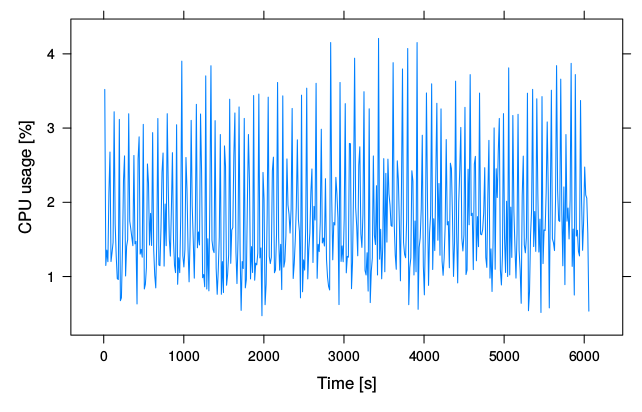
\includegraphics[width=9cm]{cpu_usage}
\centering
\caption{CPU usage during a particular simulation run}
\label{fig:cpu_usage}
\end{figure}

\begin{figure}[t]
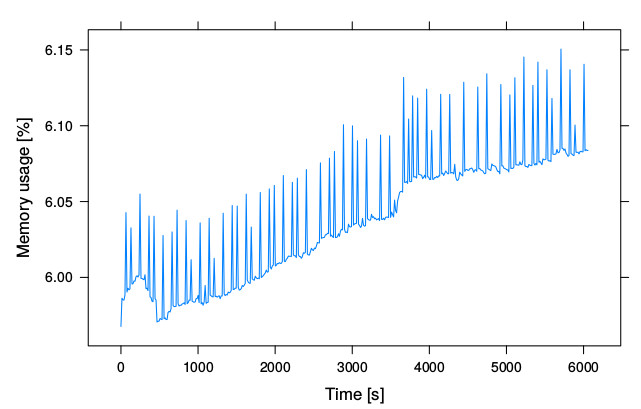
\includegraphics[width=9cm]{memory_usage}
\centering
\caption{Memory usage during a particular simulation run}
\label{fig:storage_usage}
\end{figure}

\begin{figure}[t]
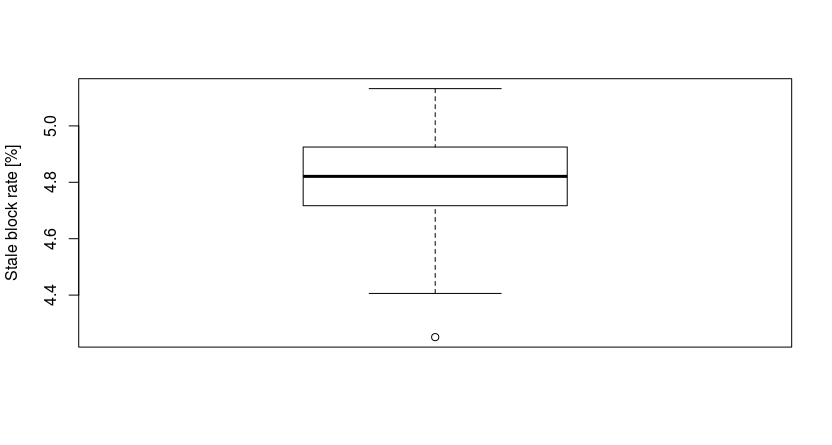
\includegraphics[width=9cm]{box_stale_rate}
\centering
\caption{Box plot of the stale block rate of 100 executions}
\label{fig:box_stale_rate}
\end{figure}

\begin{figure}[t]
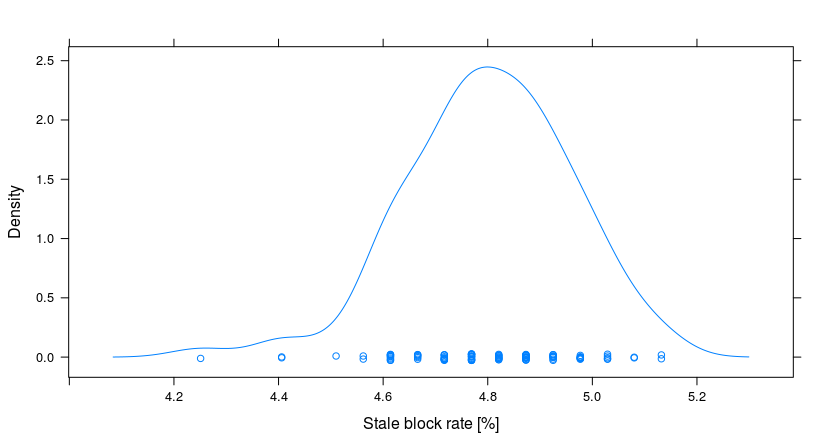
\includegraphics[width=9cm]{density_stale_rate}
\centering
\caption{Density plot of the stale block rate of 100 executions}
\label{fig:density_stale_rate}
\end{figure}
